\documentclass[10pt]{article}
\usepackage[utf8]{inputenc}
\usepackage[T1]{fontenc}
\usepackage{amsmath,amssymb}
\newcommand{\numberset}{\mathbb}
\usepackage{mathptmx}
\usepackage[italian]{babel}
\usepackage{newlfont}
\usepackage{color}
\textwidth=450pt\oddsidemargin=0pt
\usepackage{textcomp}
\usepackage{amsfonts}
\usepackage{amsthm}
\usepackage{braket}
\usepackage{bbold}
\usepackage[margin=2.8cm]{geometry}
\usepackage{fancyhdr}
\usepackage{systeme,mathtools}
\usepackage{float}
\usepackage{relsize}
\usepackage{dsfont}
\usepackage{calligra}
\usepackage{hyperref}
\usepackage{circuitikz}
\usepackage{epstopdf}
\usepackage{float}
\usepackage{listings}
\usepackage{titling}
\usepackage{graphicx}
\graphicspath{{./images/}}
\usepackage[table,xcdraw]{xcolor}

\begin{document}

\begin{titlepage}
  \begin{center}
  {{\Large{\textsc{Università degli Studi di Urbino Carlo Bo}}}} 
  \\\vspace{2mm}
  
  {\normalsize{\bf Corso di Laurea in Informatica Applicata}}
  \end{center}
  
      \vspace{40mm}
      \begin{center}
      {\Large\bf{Prodotto di differenze di valori a 4 bit}} 
      \end{center}
      
      \vspace{10mm}
      
      \begin{center}
      {\Large{Progetto d'esame di Reti Logiche 
      \vspace{3mm}}}
      \end{center}
      
      \vspace{10mm}
      
      \begin{center}
      {\Large A.A 2022/23 
      \vspace{3mm}}
      \end{center}
      
      \vspace{80mm} \par \noindent
      
  \begin{minipage}[t]{0.35\textwidth}
  %
  {\large Balducci Milena}
  \end{minipage}
  %
  \hfill
  %
  \begin{minipage}[t]{0.35\textwidth}\raggedleft \textcolor{black}{
  {\large Matricola 321791}}
  \end{minipage}
  \end{titlepage}

\newpage

\section{Specifica}

\subsection{Scopo del progetto}
L'obiettivo è quello di realizzare una rete combinatoria in tecnologia CMOS dotata di quattro ingressi A e B a 4 bit, rappresentanti quattro valori in codifica binaria naturale, 
e di una uscita Z a 8 bit che rappresenta il prodotto delle differenze dei quattro valori in ingresso.

\subsection{Specifica funzionale}
$f:{\mathbb{N}^4} \longrightarrow \mathbb{N}, \ \ f(a,b,c,d) = (a-b)\cdot (c-d)$.
\newpage

\section{Impostazione progetto a livello RT}

\subsection{Data Flow Graph}
$f = (a-b) * (a-b)$
\begin{figure}[H]
    \centering
    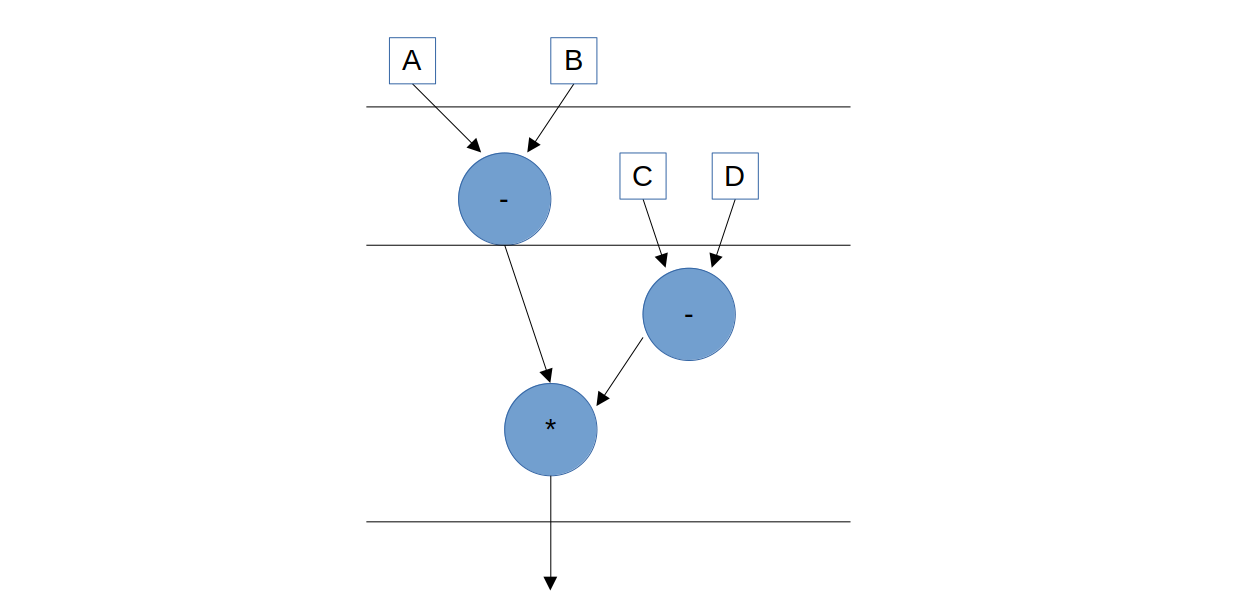
\includegraphics[width=0.8\textwidth]{dfg}
\end{figure}

Dal momento che l'operazione di sottrazione compare due volte all'interno del data flow graph, è possibile utilizzare il resource sharing, usando una unica macro aritmetica per entrambe le differenze.
Per fare questo sono necessari due cicli di clock: durante il primo viene svolta la differenza tra i primi due valori, e durante il secondo viene svolta la seconda differenza e il prodotto tra i due
risultati. 
Per svolgere la differenza tra due numeri si è scelto di utilizzare la notifica in complemento a due, che permette di svolgere le sottrazioni attraverso la somma. 
Il secondo valore andrà dunque convertito nel rispettivo complemento prima di essere passato ad un addizionatore.
\\Per mantenere i valori degli ingressi e delle uscite durante i due cicli di clock, sono necessari dei registri per gli ingressi C e D e per l'uscita di (A-B).

\subsection{Risorse}
    \begin{itemize}
        \item 3 Registri parallelo/parallelo a 4 bit
        \item 2 Multiplexer a 2 ingressi a 4 bit
        \item 1 Demultiplexer a 2 uscite a 4 bit
        \item 1 Complementatore a 4 bit
        \item 1 Addizionatore a 4 bit
        \item 1 Moltiplicatore a ingressi a 4 bit e uscita a 8 bit
    \end{itemize}
\newpage

\section{Progetto delle risorse a livello gate}
Per progettare i componenti necessari alla realizzazione della rete combinatoria illustrata nella specifica, è necessario
partire dalle porte logiche. Queste vengono realizzate partendo dai due componenti base della tecnologia C-MOS: i transistor \textbf{nMOS} e \textbf{pMOS}.
Questi due transistor sono formati da tre terminali: \textbf{Source (S)}, \textbf{Drain (D)} e \textbf{Gate (G)}.

\begin{figure}[H]
    \centering
    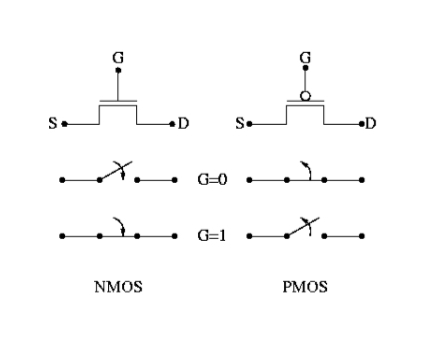
\includegraphics[width=0.8\textwidth]{transistors}
    \caption{Schema dei transistor nMOS (sinistra) e pMOS (destra)}
    \label{ }    
\end{figure}

\begin{itemize}
    \item Il transistor \textbf{nMOS} crea un collegamento tra S e D solo se il Gate assume valore 1 (alto).
    Quando viene collegato a massa, si forma la rete di \textbf{"pull-down"}.
    \item Il transistor \textbf{pMOS} collega S e D solo se il valore del Gate è 0 (basso). Quando collegato alla Vdd,
    forma quella che si chiama rete di \textbf{"pull-up"}.

\subsection{Porte logiche semplici}
Le porte logiche elementari sono quelle funzionalmente complete, ovvero che permettono di costruire tutte le altre porte logiche. 
Queste sono le porte \textbf{NOT}, \textbf{NAND} e \textbf{NOR}.

\subsubsection{Porta NOT}
La porta NOT (o inverter), corrispondente all'omonimo operatore logico, prende il segnale in ingresso e lo restituisce negato. Viene realizzata collegando pull-up e pull-down. Di seguito 
sono illustrate la tabella della verità e l'implementazione della porta NOT.
\begin{table}[ht]
    \begin{minipage}[b]{\textwidth}
    \centering
    \begin{tabular}{ | l | l |}
        \hline
           X    &    X'   \\ \hline	
           0    &    1    \\ 
           1    &    0    \\ \hline
       \end{tabular}
        \caption{Tabella della verità inverter}
        \label{table:student}
    \end{minipage}
    \end{table}
    
    \begin{figure}[H]
    \begin{minipage}[b]{\textwidth}
    
    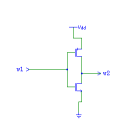
\includegraphics[width=70mm]{inverter}
    \caption{Inverter}
    \label{ }
    \end{minipage}
    \end{figure}


\subsubsection{Porta NAND}
La porta NAND è una porta logica invertente che restituisce 1 solo se almeno uno dei due ingressi vale 0, e corrisponde alla negazione della congiunzione logica dei due ingressi. 
Viene realizzata collegando in parallelo due transistor pMOS e in serie due transistor nMOS.

\begin{table}[H]
    \begin{minipage}[b]{\textwidth}
    \centering
    \begin{tabular}{|ll|l|}
    \hline
    \textbf{A} & \textbf{B} & \textbf{Y} \\ \hline
    0          & 0          & 1          \\ 
    0          & 1          & 1          \\ 
    1          & 0          & 1          \\ 
    1          & 1          & 0          \\ \hline
    \end{tabular}
        \caption{Tabella della verità NAND}
        \label{table:student}
    \end{minipage}
    \end{table}
    
    \begin{figure}[H]
    \begin{minipage}[b]{\textwidth}
    
    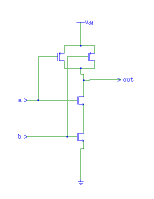
\includegraphics[width=70mm]{nand}
    \caption{Porta NAND}
    \label{ }
    \end{minipage}
    \end{figure}

\subsubsection{Porta NOR}
La porta NOR è una porta logica invertente che restituisce 1 solo se entrambi gli ingressi valgono 0, e corrisponde alla negazione della disgiunzione logica dei due ingressi. 
Viene realizzata collegando in parallelo due transistor nMOS e in serie due transistor pMOS.

\begin{table}[H]
    \begin{minipage}[b]{\textwidth}
    \centering
    \begin{tabular}{|ll|l|}
    \hline
    \textbf{A} & \textbf{B} & \textbf{Y} \\ \hline
    0          & 0          & 1          \\ 
    0          & 1          & 0          \\ 
    1          & 0          & 0          \\ 
    1          & 1          & 0          \\ \hline
    \end{tabular}
        \caption{Tabella della verità NOR}
        \label{table:student}
    \end{minipage}
    \end{table}
    
    \begin{figure}[H]
    \begin{minipage}[b]{\textwidth}
    
    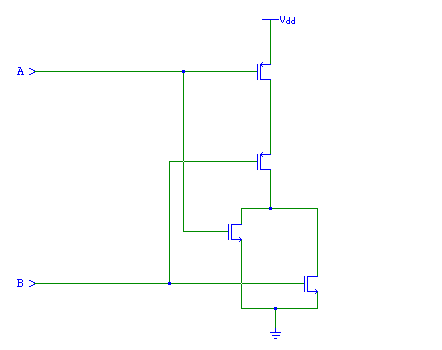
\includegraphics[width=70mm]{nor}
    \caption{Porta NOR}
    \label{ }
    \end{minipage}
    \end{figure}

\subsection{Porte logiche composte}
Le porte logiche composte utilizzate in questo progetto sono le porte AND, OR e EXOR. Ciascuna di queste è realizzata combinando porte NOT, NAND e NOR.

\subsubsection{Porta AND}
La porta AND (congiunzione logica) viene implementata tramite una porta NAND, la cui uscita viene invertita tramite una porta NOT.
\\
\textbf{(AB)=((AB)')'}
\\
\begin{table}[H]
    \begin{minipage}[b]{\textwidth}
    \centering
    \begin{tabular}{|ll|l|}
        \hline
        \textbf{A} & \textbf{B} & \textbf{AB} \\ \hline
        0          & 0          & 0           \\ \hline
        0          & 1          & 0           \\ 
        1          & 0          & 0           \\ 
        1          & 1          & 1           \\ \hline
        \end{tabular}
        \caption{Tabella della verità AND}
        \label{table:student}
    \end{minipage}
    \end{table}
    
    \begin{figure}[H]
    \begin{minipage}[b]{\textwidth}
    
    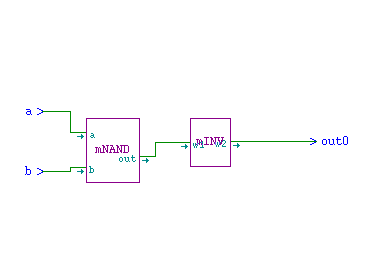
\includegraphics[width=70mm]{and}
    \caption{Porta AND}
    \label{ }
    \end{minipage}
    \end{figure}

\subsubsection{Porta OR}
E' possibile realizzare una porta OR, che corrisponde all'omonimo operatore logico, semplicemente invertendo l'uscita di una porta NOR.
\\
\textbf{(A+B)=((A+B)')'}
\\

    \begin{table}[H]
        \begin{minipage}[b]{\textwidth}
        \centering
        \begin{tabular}{|ll|l|}
            \hline
            \textbf{A} & \textbf{B} & \textbf{A + B} \\ \hline
            0          & 0          & 0              \\ \hline
            0          & 1          & 1              \\ 
            1          & 0          & 1              \\ 
            1          & 1          & 1              \\ \hline
            \end{tabular}
            \caption{Tabella della verità OR}
            \label{table:student}
        \end{minipage}
        \end{table}
        
        \begin{figure}[H]
        \begin{minipage}[b]{\textwidth}
        
        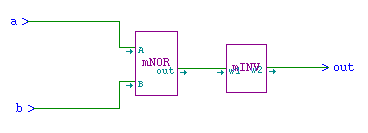
\includegraphics[width=70mm]{or}
        \caption{Porta OR}
        \label{ }
        \end{minipage}
        \end{figure}

\subsubsection{Porta EXOR}
L'operatore logico EXOR (EXclusive OR) corrisponde all'equazione logica $ab' + a'b$. Una porta logica di questo tipo è dunque realizzabile tramite porte NOT, AND e OR.
Tuttavia, utilizzando le leggi di DeMorgan è possibile realizzare questa porta logica esclusivamente tramite porte NAND e NOT. Infatti:
\\
\emph{((A'B)'(AB')')'=A'B+AB'}
\\
\begin{table}[H]
    \begin{minipage}[b]{\textwidth}
    \centering
    \begin{tabular}{|ll|l|}
        \hline
        \textbf{A} & \textbf{B} & \textbf{A'B + AB'} \\ \hline
        0          & 0          & 0                  \\ \hline
        0          & 1          & 1                  \\ 
        1          & 0          & 1                  \\
        1          & 1          & 0                  \\ \hline
        \end{tabular}
        \caption{Tabella della verità EXOR}
        \label{table:student}
    \end{minipage}
    \end{table}
    
    \begin{figure}[H]
    \begin{minipage}[b]{\textwidth}
    
    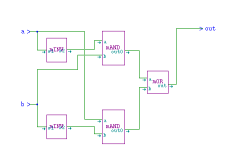
\includegraphics[width=70mm]{exor}
    \caption{Porta EXOR}
    \label{ }
    \end{minipage}
    \end{figure}
\\
\subsection{Elementi di memoria}
Gli elementi di memoria sono circuiti sequenziali che possono avere solo due stati (0 e 1) in grado di passare da uno all'altro sulla base di uno o più segnali di ingresso, e di mantenere lo stato
corrente per un periodo di tempo indefinito. Sono dunque elementi in gradi di memorizzare un singolo bit.

\subsubsection{Latch SR}
Il Latch SR (Set-Reset) è un elemento di memoria asincrono dotato di due segnali di ingresso \textbf{\emph{s}} e \textbf{\emph{r}} e di due porte NOR, ciascuna avente un ingresso collegato a 
\emph{s} o \emph{r}, e l'altro collegato all'uscita dell'altra porta NOR.
Il Latch SR ammette un cambiamento di stato sulla sola base dei segnali di ingresso:
\begin{itemize}
    \item Con \emph{s}=1, \emph{r}=0 si passa allo stato di \textbf{SET}: \emph{y}'=0, \emph{y}=1;
    \item Con \emph{s}=0, \emph{r}=1 si passa allo stato di \textbf{RESET}: \emph{y}'=1, \emph{y}=0;
    \item Con \emph{s}=0, \emph{r}=0 lo stato rimane invariato (\textbf{HOLD}).
\end{itemize}
La configurazione \emph{s}=1, \emph{r}=1 non è ammessa. 

\begin{table}[H]
    \begin{minipage}[b]{\textwidth}
    \centering
    \begin{tabular}{|lll|ll|}
        \hline
        \textbf{y'} & \textbf{s} & \textbf{r} & \textbf{f (y)} & \textbf{g (y')} \\ \hline
        0           & 0          & 0          & 1              & 0               \\ 
        0           & 0          & 1          & 0              & 1               \\ 
        0           & 1          & 0          & 1              & 0               \\ 
        0           & 1          & 1          & 0              & 0               \\ 
        1           & 0          & 0          & 0              & 1               \\ 
        1           & 0          & 1          & 0              & 1               \\ 
        1           & 1          & 0          & 1              & 0               \\ 
        1           & 1          & 1          & 0              & 0               \\ \hline
        \end{tabular}
        \caption{Tabella della verità Latch SR}
        \label{tab:my-table}
    \end{minipage}
\end{table}

Il problema legato a questa rete sequenziale, che è asincrona, è la possibilità che si presentino situazioni transitorie che potrebbero modificare le configurazioni degli ingressi in maniera non desiderata o 
non prevedibile.

\subsubsection{Flip-flop SR}
Nel Flip-flop SR, i due segnali \emph{s} e \emph{r} sono generati da due porte AND, alle quali sono collegati due segnali di ingresso \textbf{\emph{S}} ed \textbf{\emph{R}} 
e un segnale di sincronismo denominato \textbf{Clock}, di natura generalmente periodica. 
In questo modo, ci si assicura che l'aggiornamento degli stati avvenga solo in momenti ben definiti.
\begin{itemize}
    \item con Clock=1, \emph{S}=1, \emph{R}=0 si ha lo stato di \textbf{SET};
    \item con Clock=1, \emph{S}=0, \emph{R}=1 si ha lo stato di \textbf{RESET};
    \item con Clock=1, \emph{S}=0, \emph{R}=0 si ha lo stato di \textbf{HOLD};
    \item con Clock=0, il flip-flop rimane in stato di HOLD indipendentemente dalla configurazione degli ingressi.
\end{itemize}

\begin{table}[H]
    \begin{minipage}[b]{\textwidth}
    \centering
    \begin{tabular}{|lll|ll|l|}
        \hline
        \textbf{Clk} & \textbf{S} & \textbf{R} & \textbf{s} & \textbf{r} &       \\ \hline
        0            & 0          & 0          & 0          & 0          & HOLD  \\ 
        0            & 0          & 1          & 0          & 0          & HOLD  \\ 
        0            & 1          & 0          & 0          & 0          & HOLD  \\ 
        0            & 1          & 1          & 0          & 0          & HOLD  \\ 
        1            & 0          & 0          & 0          & 0          & HOLD  \\ 
        1            & 0          & 1          & 0          & 1          & RESET \\ 
        1            & 1          & 0          & 1          & 0          & SET   \\ 
        1            & 1          & 1          & 1          & 1          & N.A.  \\ \hline
        \end{tabular}
        \caption{Tabella della verità Flip-flop SR}
        \label{tab:my-table}
    \end{minipage}
    \end{table}

\subsubsection{Flip-flop D-level sensitive}
Il funzionamento di un Flip-flop D-level sensitive è analogo a quello del FFSR, ma ai due segnali \emph{S} e \emph{R} viene sostituito un unico segnale \emph{D}: 
\emph{S} corrisponde a \emph{D}, \emph{R} a \emph{D'}. Questo permette di escludere la configurazione non ammessa \emph{s}=1, \emph{r}=1, 
e di avere durante il periodo di salita del clock due sole configurazioni possibili, ovvero quelle di SET e di RESET. 
Il FFDls rimane sensibile alle variazioni degli ingressi per tutta la durata di attività del segnale di clock.

\begin{table}[H]
    \begin{minipage}[b]{\textwidth}
    \centering
    \begin{tabular}{|ll|ll|ll|l|}
        \hline
        \textbf{Clk} & \textbf{D} & \textbf{S} & \textbf{R} & \textbf{s} & \textbf{r} &       \\ \hline
        0            & 0          & 0          & 1          & 0          & 0          & HOLD  \\ 
        0            & 1          & 1          & 0          & 0          & 0          & HOLD  \\ 
        1            & 0          & 0          & 1          & 0          & 1          & RESET \\ 
        1            & 1          & 1          & 0          & 1          & 0          & SET   \\ \hline
        \end{tabular}
        \caption{Tabella della verità FF D-level sensitive}
        \label{tab:my-table}
    \end{minipage}
    \end{table}
    
    \begin{figure}[H]
    \begin{minipage}[b]{\textwidth}
    \centering
    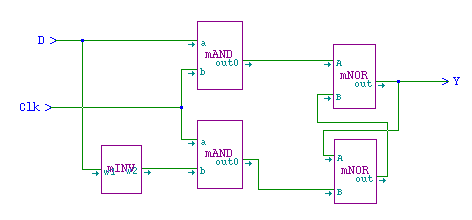
\includegraphics[width=100mm]{ffdls}
    \caption{Flip-flop D-level sensitive}
    \label{ }
    \end{minipage}
    \end{figure}


\subsubsection{Flip-flop D-edge triggered}
Il Flip-flop D-edge triggered è un elemento di memoria nel quale l'aggiornamento dello stato è consentito solo sul fronte di salita del clock. E' costruito tramite due FFDls, 
denominati \textbf{master} e \textbf{slave}.
Il \emph{master} prende in ingresso il segnale di clock negato e il bit da memorizzare, \emph{slave} mentre lo slave riceve l'uscita del \emph{master} e il segnale di clock. 

\begin{itemize}
    \item Quando Clock=0, il \emph{master} è abilitato a cambiare stato mentre lo \emph{slave} mantiene le uscite stabili;
    \item Quando Clock=1, lo \emph{slave} rileva le variazioni di stato del \emph{master} e le propaga, mentre il \emph{master} è insensibile alle variazioni degli ingressi.
\end{itemize}

\begin{figure}[H]
    \begin{minipage}[b]{\textwidth}
    \centering
    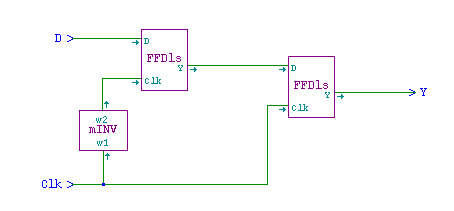
\includegraphics[width=100mm]{ffdet}
    \caption{Flip-flop D edge-triggered}
    \label{ }
    \end{minipage}
    \end{figure}

\subsection{Registri}
Un registro è un elemento di memoria in grado di memorizzare vettori di $n$ bit. Ne esistono di differenti tipi, quelli utilizzati in questo progetto sono registri parallelo/parallelo a 4 bit.
Questo tipo di registri è dotato di quattro FFD-edge triggered. Tutti i bit vengono ricevuti in ingresso contemporaneamente, collegando l'ingresso dell'$i$-esimo flip-flop all'$i$-esimo bit del 
vettore in ingresso, e le uscite vengono tutte lette contemporaneamente. 

\begin{figure}[H]
    \begin{minipage}[b]{\textwidth}
    \centering
    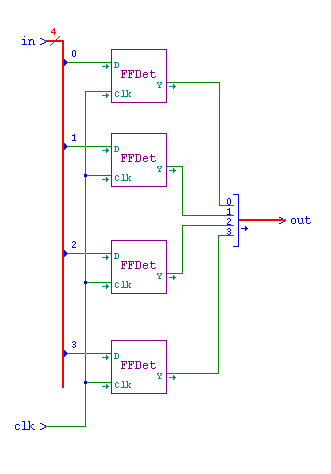
\includegraphics[width=70mm]{reg4}
    \caption{Registro parallelo/parallelo a 4 bit}
    \label{ }
    \end{minipage}
    \end{figure}

\subsection{Multiplexer}
Il Multiplexer (MUX) è un componente combinatorio dotato di $x$ ingressi a $n$ bit e di una uscita a $n$ bit, in grado di scegliere il valore che assumerà l'uscita tra quelli in ingresso sulla base di uno o più segnali
di controllo. Il più semplice multiplexer ha 2 ingressi a 1 bit e una uscita a un bit. Funzione, tabella della verità e implementazione sono illustrati di seguito:

$f(a,b,c) = ac' + bc$

\begin{table}[H]
    \begin{minipage}[b]{\textwidth}
    \centering
        \begin{tabular}{|lll|l|}
        \hline
        \textbf{A} & \textbf{B} & \textbf{C} & \textbf{F} \\ \hline
        0          & 0          & 0          & 0          \\ 
        0          & 0          & 1          & 0          \\ 
        0          & 1          & 0          & 0          \\ 
        0          & 1          & 1          & 1          \\ 
        1          & 0          & 0          & 1          \\ 
        1          & 0          & 1          & 0          \\ 
        1          & 1          & 0          & 1          \\ 
        1          & 1          & 1          & 1          \\ \hline
        \end{tabular}
        \caption{Tabella della verità MUX}
        \label{tab:my-table}
    \end{minipage}
    \end{table}
    
    \begin{figure}[H]
    \begin{minipage}[b]{\textwidth}
    \centering
    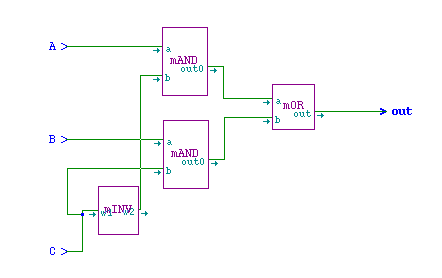
\includegraphics[width=100mm]{mux1}
    \caption{Multiplexer a 1 bit}
    \label{ }
    \end{minipage}
    \end{figure}

E' possibile realizzare MUX in grado di scegliere tra due valori a $n$ bit combinando $n$ MUX a 1 bit, ognuno dei quali seleziona
l'$i$-esimo bit del primo o del secondo ingresso a seconda del segnale di controllo. In questo progetto è stato fatto uso di MUX con due ingressi a 4 bit e una uscita a 4 bit. 

\begin{figure}[H]
    \begin{minipage}[b]{\textwidth}
        \centering
        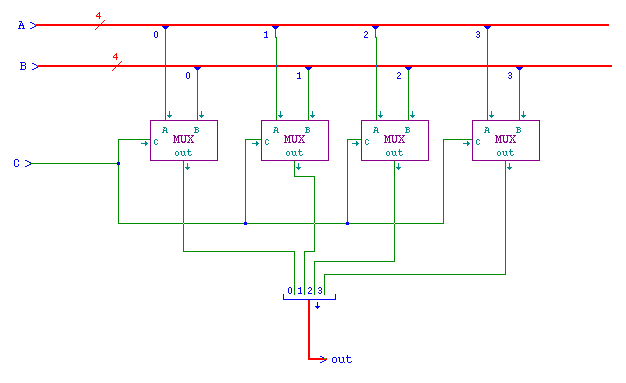
\includegraphics[width=\textwidth]{mux4}
        \caption{Multiplexer a 4 bit}
        \label{ }
    \end{minipage}
\end{figure}

\subsection{Demultiplexer}
Un Demultiplexer (DEMUX) è un componente che funziona in maniera opposta a un MUX: è dotato di un ingresso a $n$ bit e di $x$ uscite a $n$ bit; una di queste uscite assume il valore dell'ingresso,
mentre le altre valgono zero. La selezione è operata sulla base di uno o più segnali di controllo.
Il più semplice DEMUX, illustrato di seguito, è dotato di un ingresso a 1 bit e due uscite a 1 bit.
\\
$f_1 = ac'\\
f_2 = ac$
\\
\begin{table}[H]
    \begin{minipage}[b]{\textwidth}
    \centering
        \begin{tabular}{|ll|ll|}
        \hline
        \textbf{A} & \textbf{C} & \textbf{F1} & \textbf{F2} \\ \hline
        0          & 0          & 0           & 0           \\ 
        0          & 1          & 0           & 0           \\ 
        1          & 0          & 1           & 0          \\ 
        1          & 1          & 0           & 1           \\ \hline
        \end{tabular}
        \caption{Tabella della verità DEMUX}
        \label{tab:my-table}
    \end{minipage}
    \end{table}
    
    \begin{figure}[H]
    \begin{minipage}[b]{\textwidth}
    \centering
    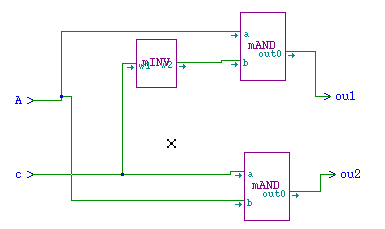
\includegraphics[width=70mm]{demux1}
    \caption{Demultiplexer a 1 bit}
    \label{ }
    \end{minipage}
    \end{figure}

Come per i multiplexer, è possibile implementare un DEMUX con due uscite a $n$ bit combinando $n$ DEMUX a 1 bit, ciascuno dei quali prende in ingresso l'$i$-esimo bit del vettore in ingresso.
Il DEMUX raffigurato di seguito è dotato di un ingresso e due uscite a 4 bit.

\begin{figure}[H]
    \begin{minipage}[b]{\textwidth}
        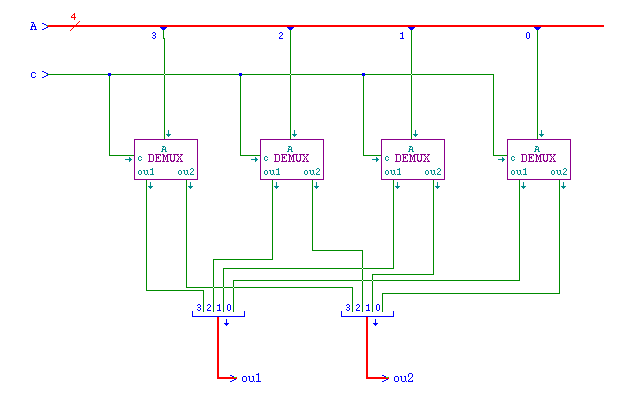
\includegraphics[width=\textwidth]{demux4}
        \caption{Demultiplexer a 4 bit}
        \label{ }
    \end{minipage}
\end{figure}

\subsection{Macro aritmetiche}
\subsubsection{Half adder}
Un Half Adder (HA) è una rete combinatoria in grado di calcolare la somma di due bit. E' dotato di due ingressi a un bit (gli addendi) e di due uscite S e Cout che rappresentano Il
risultato della somma e il riporto in uscita, rispettivamente.
Le equazioni corrispondenti alle due uscite sono:\\
$S = A \oplus Cin$\\
$Cout = ACin$

\begin{table}[H]
    \begin{minipage}[b]{\textwidth}
    \centering
    \begin{tabular}{|l|l|l|l|}
        \hline
        \textbf{A} & \textbf{Cin} & \textbf{S} & \textbf{Cout} \\ \hline
        0          & 0            & 0          & 0             \\ 
        0          & 1            & 1          & 0             \\ 
        1          & 0            & 1          & 0             \\ 
        1          & 1            & 0          & 1             \\ \hline
        \end{tabular}
        \caption{Tabella della verità HA}
        \label{table:student}
    \end{minipage}
    \end{table}
    
    \begin{figure}[H]
    \begin{minipage}[b]{\textwidth}
    \centering
    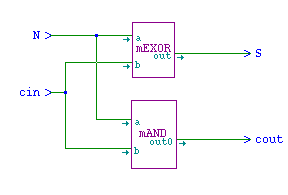
\includegraphics[width=70mm]{ha}
    \caption{Half Adder}
    \label{ }
    \end{minipage}
    \end{figure}

\subsubsection{Full adder}
Un Full Adder (FA) è una rete combinatoria che calcola la somma di tre bit. E' dotato di tre ingressi A, B e Cin che rappresentano il primo addendo, il seccondo addendo e il riporto
in ingresso, e di due uscite S e Cout che rappresentano il risultato della somma e il riporto in uscita, rispettivamente. 
Le equazioni delle due uscite sono:\\
$
S = Cin \oplus (A \oplus B)\\
cout = AB + Cin(A + B)
$\\
E' possibile implementare questo componente utilizzando due HA in cascata e una porta NOT. Il primo HA calcola la somma dei due addendi, e al risultato viene sommato il riporto in ingresso
tramite il secondo HA.
Il riporto in uscita del FA corrisponde alla disgiunzione logica dei riporti in uscita dei due HA.

\begin{table}[H]
    \begin{minipage}[b]{\textwidth}
    \centering
    \begin{tabular}{|l|l|l|l|l|}
        \hline
        \textbf{A} & \textbf{B} & \textbf{Cin} & \textbf{S} & \textbf{Cout} \\ \hline
        0          & 0          & 0            & 0          & 0             \\ 
        0          & 0          & 1            & 1          & 0             \\ 
        0          & 1          & 0            & 1          & 0             \\ 
        0          & 1          & 1            & 0          & 1             \\ 
        1          & 0          & 0            & 1          & 0             \\ 
        1          & 0          & 1            & 0          & 1             \\ 
        1          & 1          & 0            & 0          & 1             \\ 
        1          & 1          & 1            & 1          & 1             \\ \hline
        \end{tabular}
        \caption{Tabella della verità FA}
        \label{table:student}
    \end{minipage}
    \end{table}
    
    \begin{figure}[H]
    \begin{minipage}[b]{\textwidth}
    \centering
    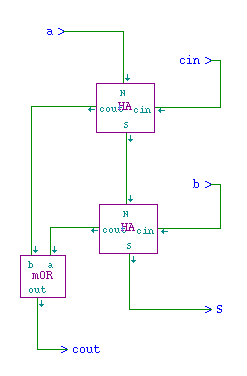
\includegraphics[width=70mm]{FA}
    \caption{Full Adder}
    \label{ }
    \end{minipage}
    \end{figure}

\subsubsection{Complementatore}
Per convertire un numero intero nel rispettivo complemento a 2, è sufficiente complementare i singoli bit che lo compongono, e poi sommare 1 al vettore di bit così ottenuto.
Per realizzare un circuito in grado di svolgere questa operazione per valori a 4 bit si utilizzando dunque degli inverter, le cui uscite vanno in ingresso a degli HA in cascata.
Il riporto in ingresso del primo HA viene collegato alla differenza di potenziale.

\begin{figure}[H]
    \begin{minipage}[c]{\textwidth}
    \centering    
    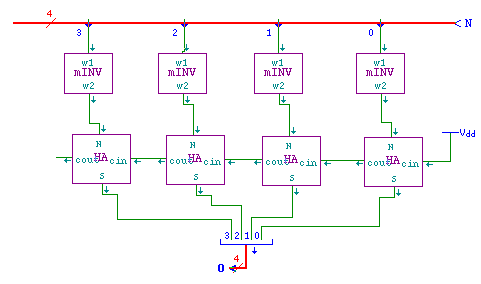
\includegraphics[width=\textwidth]{complementoadue}
    \caption{Complementatore a 4 bit}
    \label{ }
    \end{minipage}
\end{figure}


\subsubsection{RCA a 4bit}
Un Ripple Carry Adder (RCA) è una macro funzionale per l'addizione di valori a $n$bit. Il suo funzionamento si basa sullo schema classico dell'addizione in colonna:

\begin{table}[H]
    \begin{minipage}[b]{\textwidth}
    \centering
    \begin{tabular}{rrrrrr}
       & \textbf{c3} & \textbf{c2} & \textbf{c1} & \textbf{c0} &   \\ \hline
       & x3          & x2          & x1          & x0          & + \\ 
       & y3          & y2          & y1          & y0          & = \\ \hline
    c4 & s3          & s2          & s1          & s0          &   \\
    \end{tabular}
    \caption{Schema addizione in colonna}
    \label{tab:my-table}
    \end{minipage}
\end{table}

Questo schema viene implementato tramite FA, collegando il riporto in ingresso di ogni FA al riporto in uscita del FA precedente, con l'eccezione del primo FA, il cui riporto in ingresso è
collegato alla massa.

\begin{figure}[H]
    \begin{minipage}[c]{\textwidth} 
    \centering   
    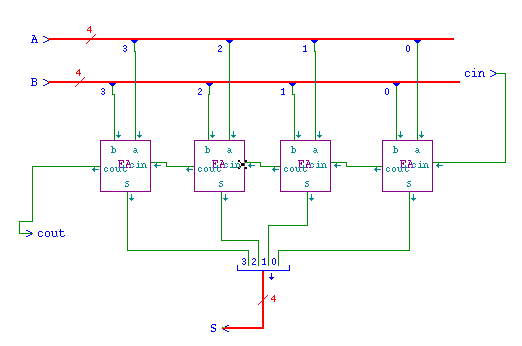
\includegraphics[width=\textwidth]{RCA}
    \caption{Ripple-Carry Adder a 4 bit}
    \label{ }
    \end{minipage}
\end{figure}


\subsubsection{Moltiplicatore a 4 bit}
Un moltiplicatore è, come suggerisce il nome, un componente combinatorio in grado di effettuare il prodotto di valori a $n$ bit. In questo progetto è stato utilizzato un moltiplicatore a 4 bit.
Per costruire questo componente, è necessario innanzitutto ricavare la funzione logica del prodotto tra due bit. Osservando la tabella della verità sottostante, risulta evidente che questa corrisponde
al prodotto logico di due bit, e dunque la funzione logica della moltiplicazione è \textbf{S=AB}.

\begin{table}[H]
    \begin{minipage}[c]{\textwidth}
    \centering
    \begin{tabular}{|ll|l|}
    \hline
    \textbf{A} & \textbf{B} & \textbf{S} \\ \hline
    0          & 0          & 0          \\ 
    0          & 1          & 0          \\ 
    1          & 0          & 0          \\ 
    1          & 1          & 1          \\ \hline
    \end{tabular}
    \caption{Tabella della verità moltiplicazione 1 bit}
    \label{tab:my-table}
    \end{minipage}
    \end{table}

Una volta determinata la funzione del prodotto matematico tra due bit, per realizzare un moltiplicatore è sufficiente seguire il classico schema della moltiplicazione in colonna.

\begin{table}[H]
    \begin{minipage}[c]{\textwidth}
    \centering
    \begin{tabular}{rrrrrrrrr}
       &       &       &       & x3    & x2    & x1    & x0    & * \\ 
       &       &       &       & y3    & y2    & y1    & y0    & = \\ \hline
       & 0     & 0     & 0     & y0x3  & y0x2  & y0x1  & y0x0  & + \\ 
       & 0     & 0     & y1x3  & y1x2  & y1x1  & y1x0  & 0     & + \\ 
       & 0     & y2x3  & y2x2  & y2x1  & y2x0  & 0     & 0     & + \\ 
       & y3x3  & y3x2  & y3x1  & y3x0  & 0     & 0     & 0     & + \\ \hline
    s7 & s6    & s5    & s4    & s3    & s2    & s1    & s0    &   \\ 
    \end{tabular}
    \caption{Schema moltiplicazione in colonna}
    \label{tab:my-table}
    \end{minipage}
\end{table}

Seguendo questo schema, è possibile implementare il moltiplicatore utilizzando delle porte AND per svolgere il prodotto dei singoli bit, e poi FA e HA per sommare tra loro i prodotti parziali che si
trovano lungo la stessa colonna, prestando attenzione a propagare correttamente il riporto in uscita alla colonna successiva. 

\begin{figure}[H]
    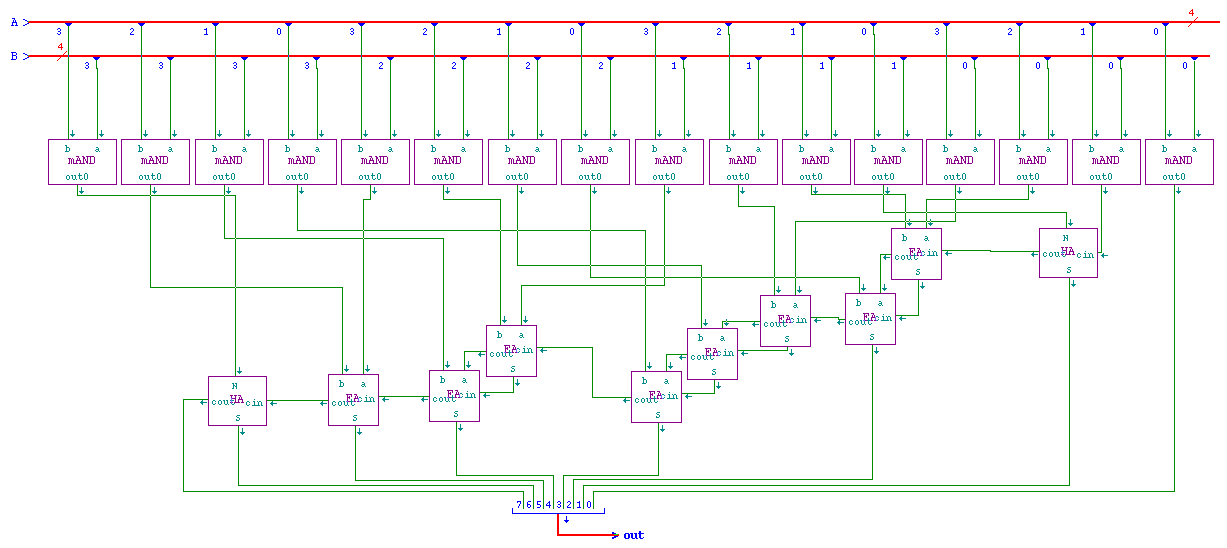
\includegraphics[width=\textwidth]{MUL}
    \centering
\end{figure}


\section{Data Path}
\begin{figure}[H]
    \centering
    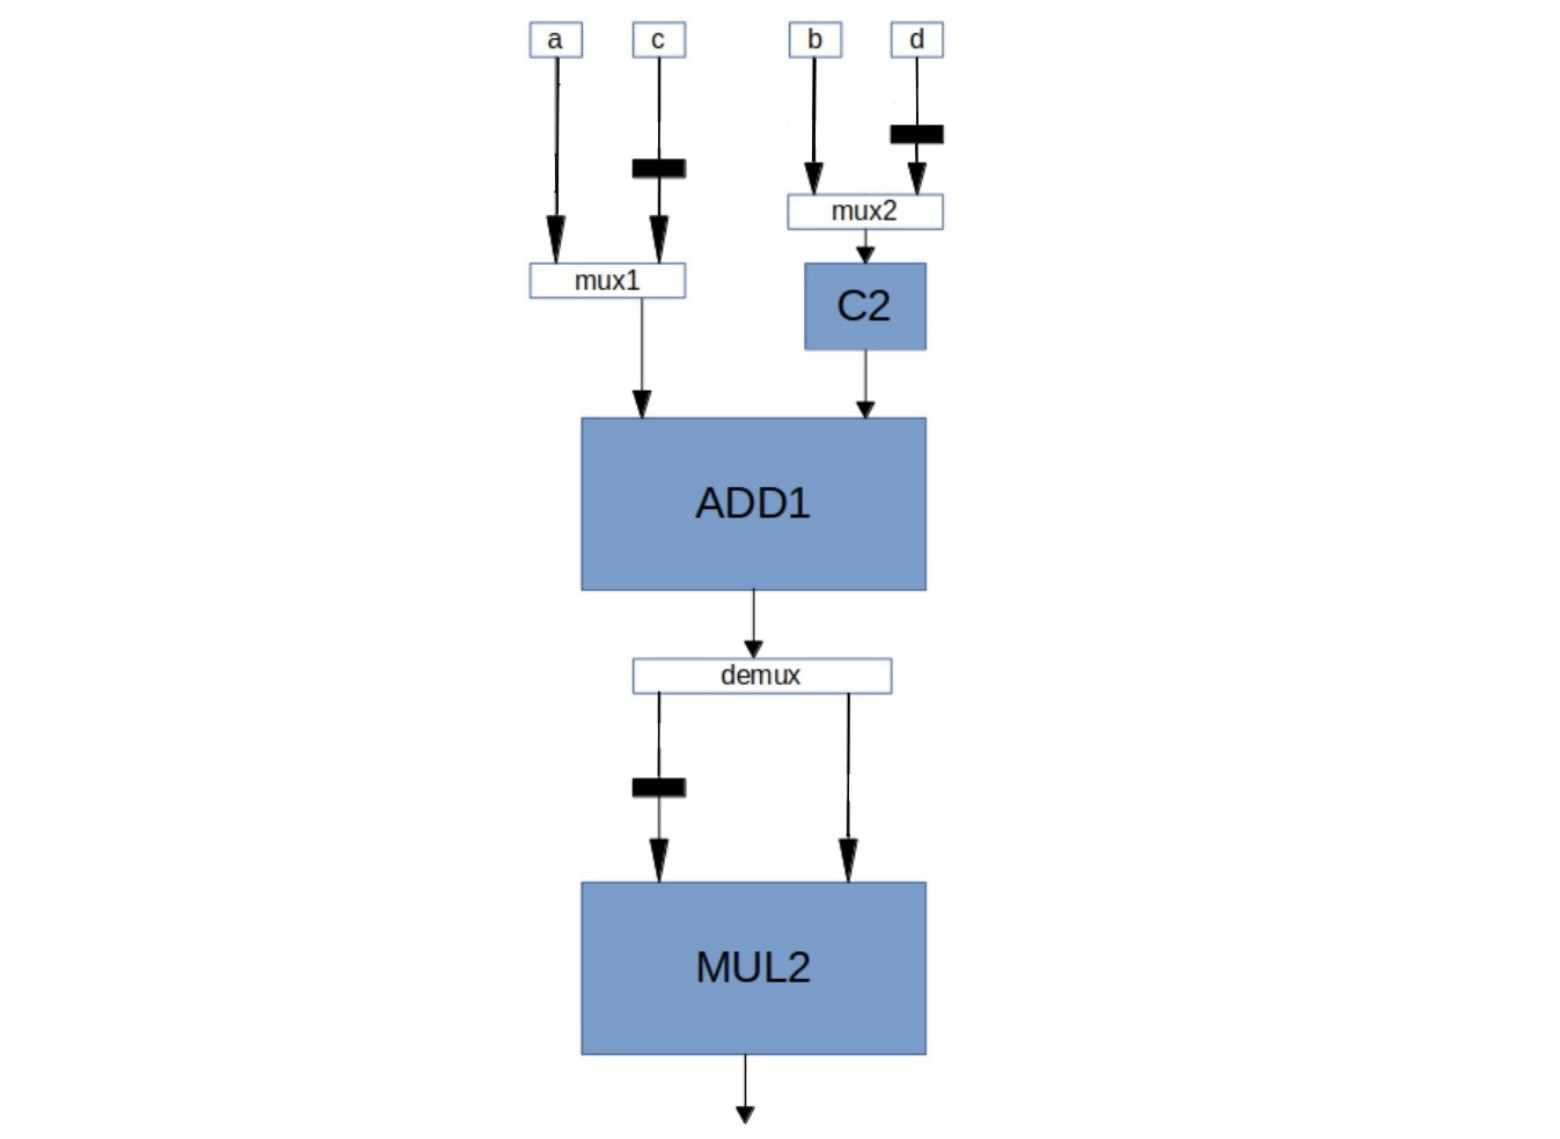
\includegraphics[width=0.7\textwidth]{datapath}
\end{figure}


\section{Control Unit}

\subsection{Specifica}
Il circuito che si sta progettando necessita di due multiplexer e un demultiplexer, tutti con un singolo segnale di controllo; e di due cicli di clock.
Durante il primo ciclo di clock, tutti e tre i componenti devono selezionare l'ingresso/uscita di sinistra (0), mentre nel secondo ciclo di clock viene selezionato l'ingresso/uscita
di destra (1).
Dal momento che per tutti e tre i componenti controllati dalla CU il segnale assume lo stesso valore all'interno del medesimo ciclo di clock, è possibile utilizzare un unico segnale
di controllo (denominato C).

\begin{table}[H]
    \begin{minipage}[c]{\textwidth}
    \centering
    \begin{tabular}{|c|ccc|c|}
        \hline
        \textbf{Ciclo di Clock} & \textbf{MUX1} & \textbf{MUX2} & \textbf{DEMUX} & \textbf{C}\\ \hline
        0                       & 0             & 0             & 0              & 0         \\ 
        1                       & 1             & 1             & 1              & 1         \\ \hline
        \end{tabular}
    \end{minipage}
    \end{table}

E' possibile implementare questa specifica tramite una macchina a stati finiti che può assumere due stati (Ciclo 0 e Ciclo 1) e produce un unico segnale in uscita. 
La funzione di uscita dipende unicamente dallo stato presente, mentre la funzione di stato futuro dipende dallo stato presente e dagli ingressi.

\begin{figure}[H]
    \centering
    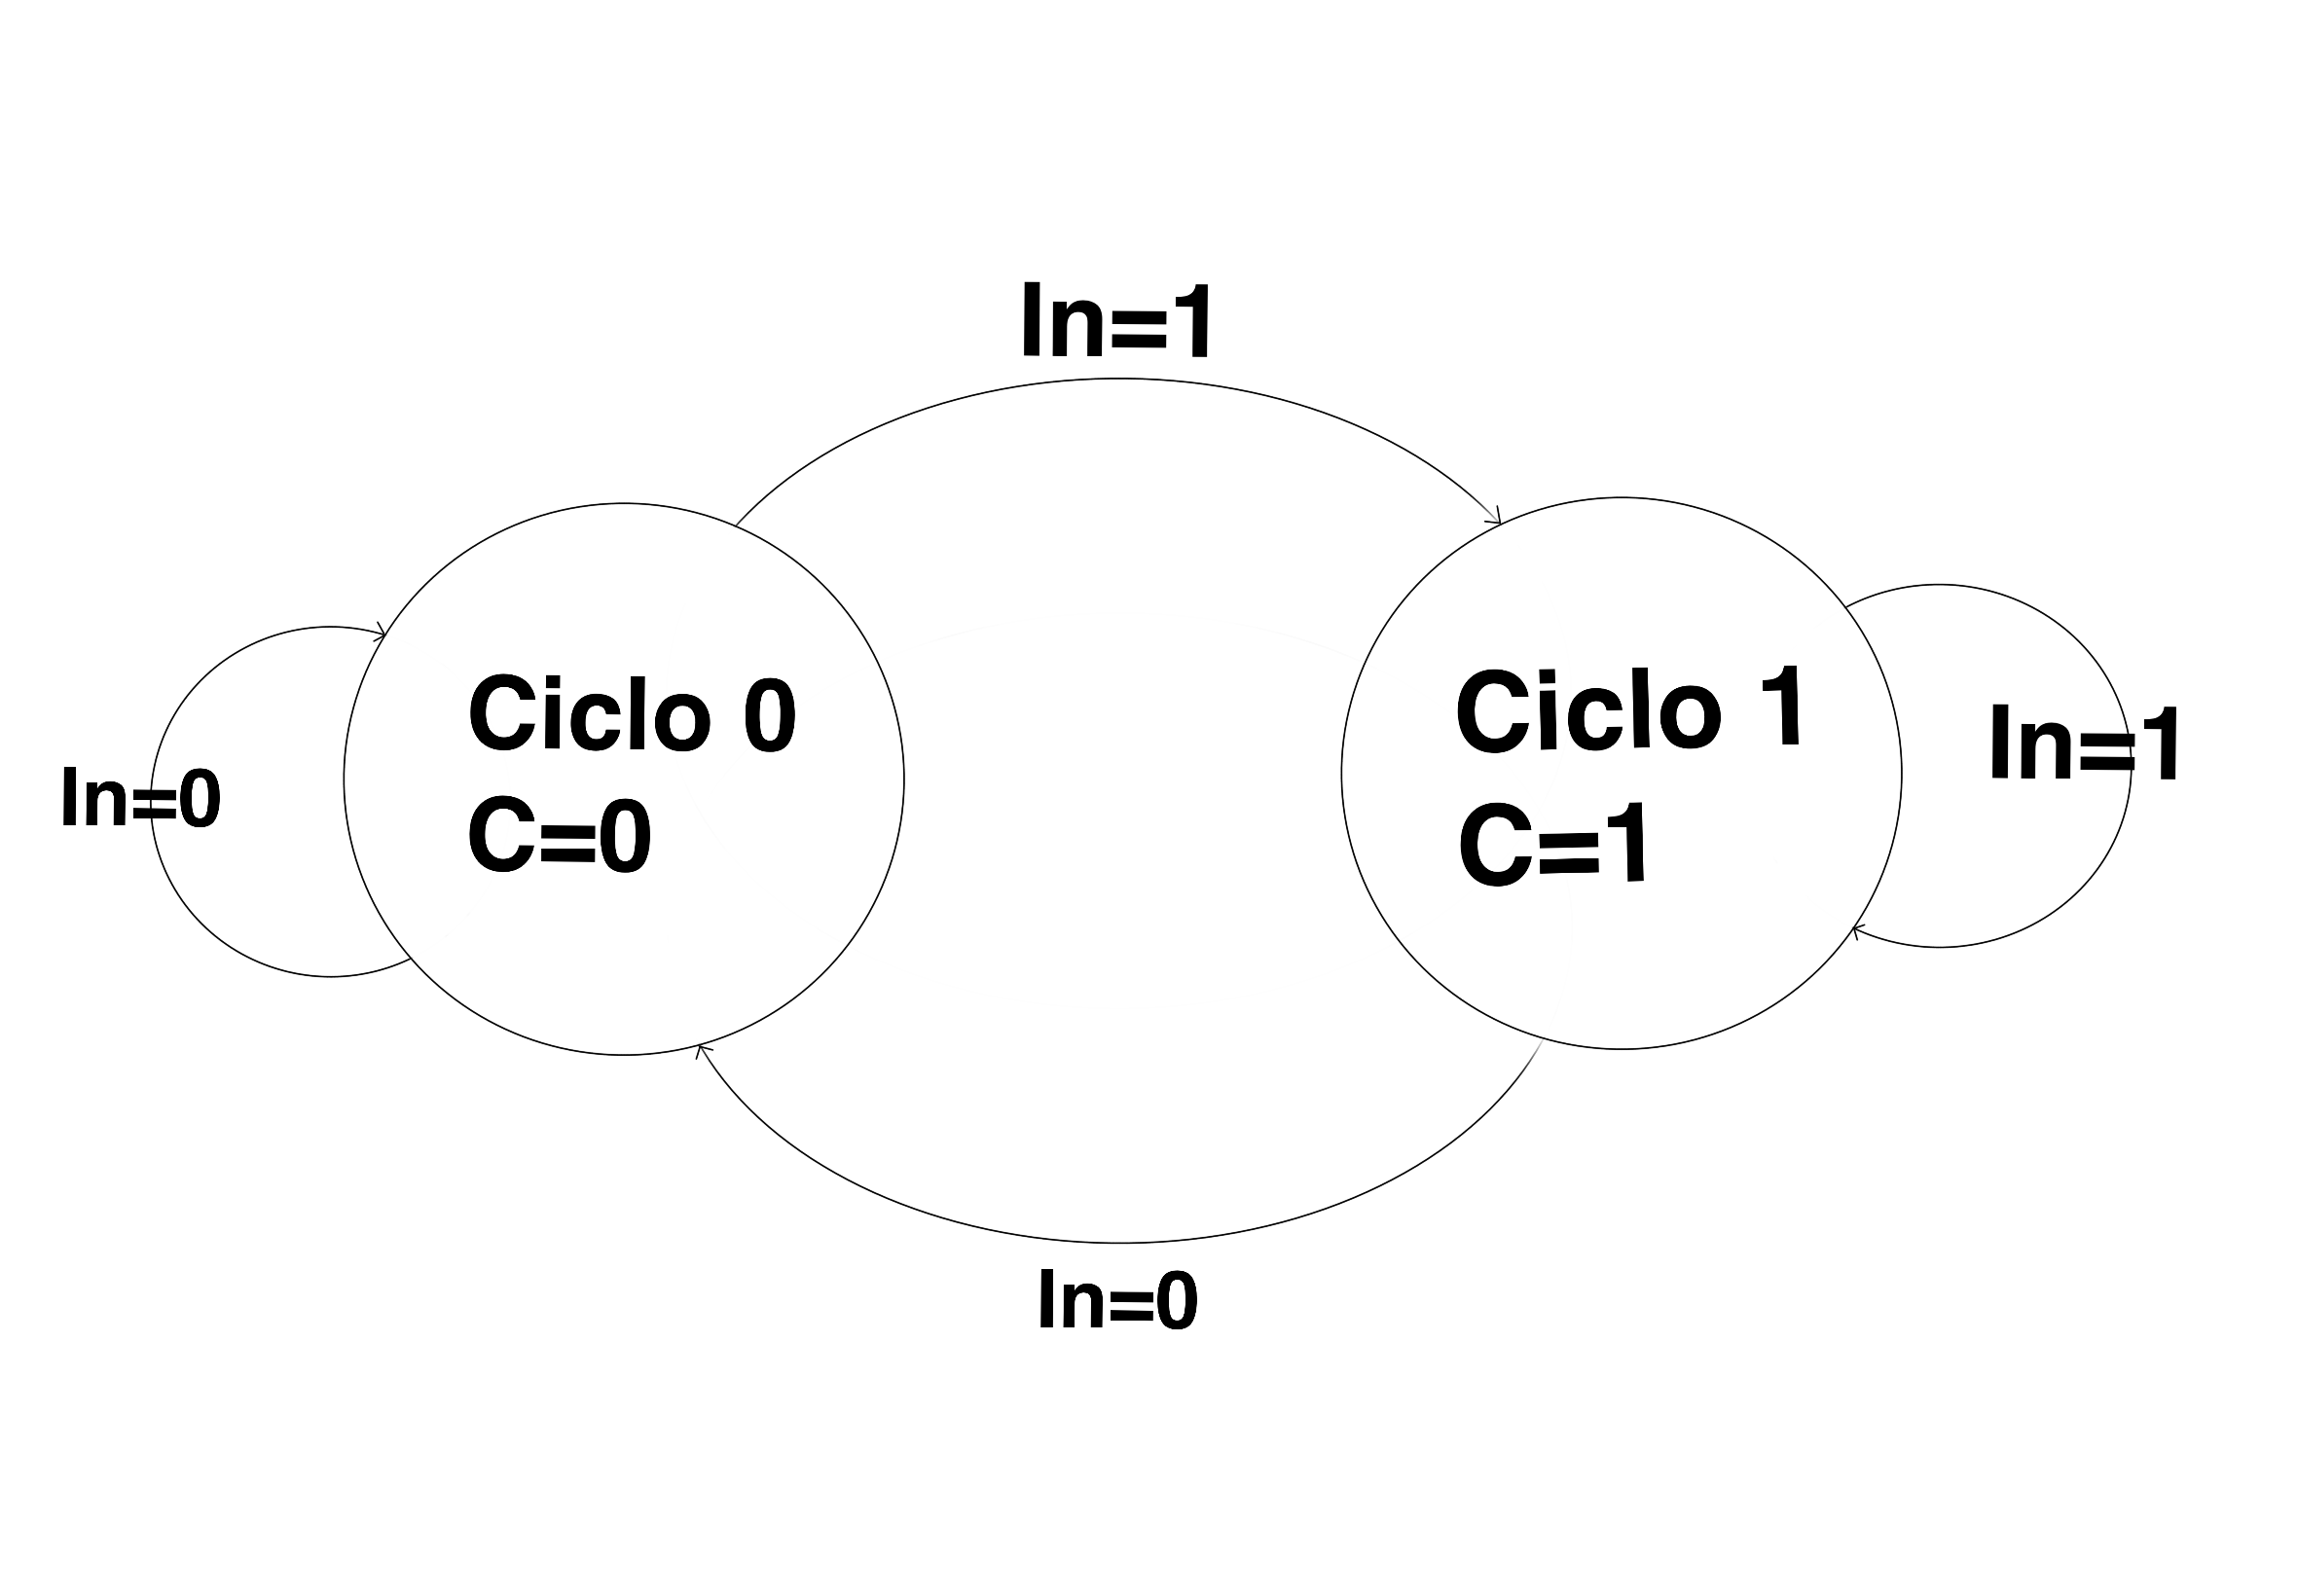
\includegraphics[width=0.7\textwidth]{statediag}
\end{figure}


\subsection{Implementazione della macchina di Moore}
Dal momento che la funzione di uscita dipende unicamente dallo stato presente, è possibile implementare la control unit come una macchina di Moore.
I due stati della macchina di Moore possono essere codificati con un singolo bit S, e l'ingresso è a sua volta rappresentato da un segnale ad un singolo bit.
\begin{table}[H]
    \begin{minipage}[c]{\textwidth}
    \centering
    \begin{tabular}{|c|c|c|c|}
        \hline
        \textbf{In} &\textbf{S}  & \textbf{C} & \textbf{Sn} \\ \hline
        0           &0           & 0          & 0           \\
        0           &1           & 1          & 0           \\
        1           &0           & 0          & 1           \\ 
        1           &1           & 1          & 0           \\ \hline
        \end{tabular}
    \end{minipage}
    \end{table}

Le funzioni di uscita e stato futuro risultano dunque essere:
\\
\textbf{Sn = InS'}\\ 
\textbf{C = In'S + InS = S}
\\
\\
Lo stato presente viene conservato tramite un FFD-edge triggered,
che viene aggiornato solo sul fronte di salita del clock (che in questo caso è rappresentato da un interrutore manovrato manualmente). 
\\
\\
\begin{figure}[ht]
    \begin{minipage}[c]{\textwidth}
    \centering
    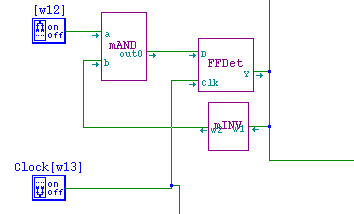
\includegraphics[width=70mm]{cu}
    \caption{Control Unit}
    \label{ }
    \end{minipage}
\end{figure}

\newpage

\section{Simulazione e analisi del progetto}
\subsection{Verifica funzionale}
In questa sezione sono riportate delle immagini illustrative di alcune simulazioni effettuate per testare la funzionalità del circuito. In tutto sono riportate tre simulazioni, per ciascuna vengono 
illustrati entrambi i cicli di clock.

\begin{figure}[H]
    \begin{minipage}[c]{\textwidth}
    \centering    
    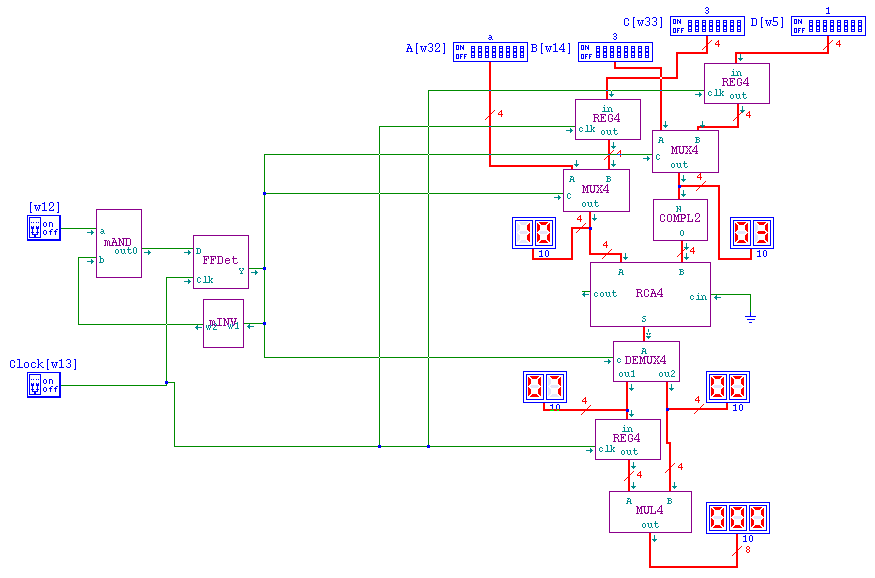
\includegraphics[width=\textwidth]{s1c0}
    \caption{Simulazione 1: ciclo di clock 0}
    \label{ }
    \end{minipage}
\end{figure}

\begin{figure}[H]
    \begin{minipage}[c]{\textwidth}
    \centering
    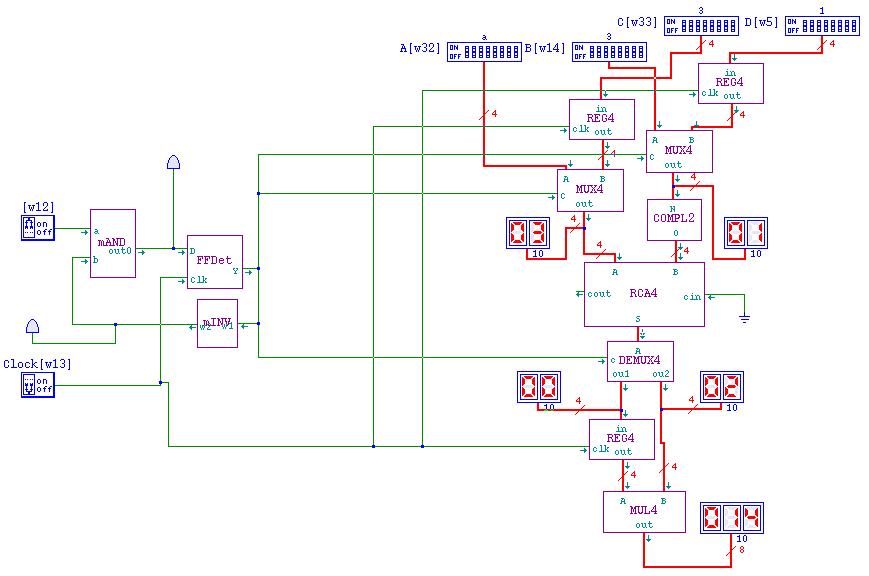
\includegraphics[width=\textwidth]{s1c1}
    \caption{Simulazione 1: ciclo di clock 1}
    \label{ }
    \end{minipage}
\end{figure}

\begin{figure}[H]
    \begin{minipage}[c]{\textwidth}
    \centering
    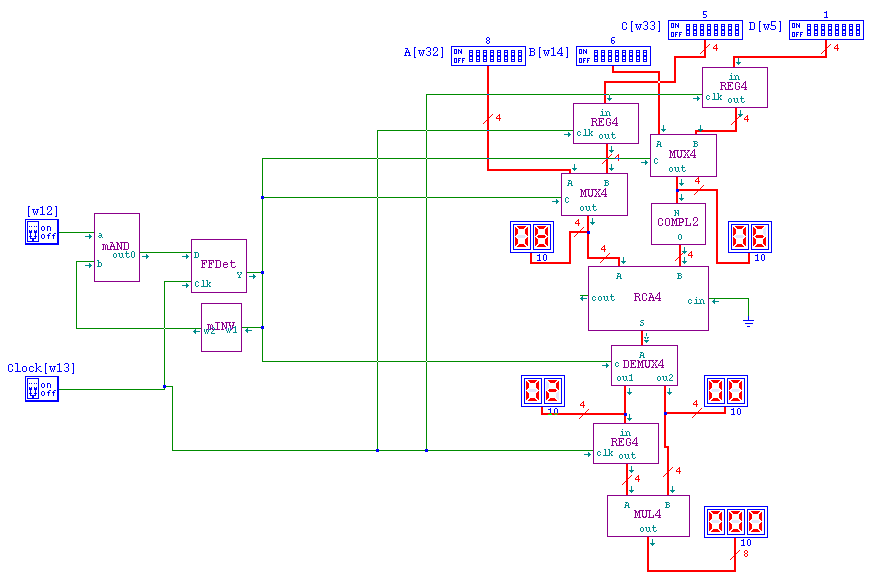
\includegraphics[width=\textwidth]{s2c0}
    \caption{Simulazione 2: ciclo di clock 0}
    \label{ }
    \end{minipage}
\end{figure}

\begin{figure}[H]
    \begin{minipage}[c]{\textwidth}
    \centering
    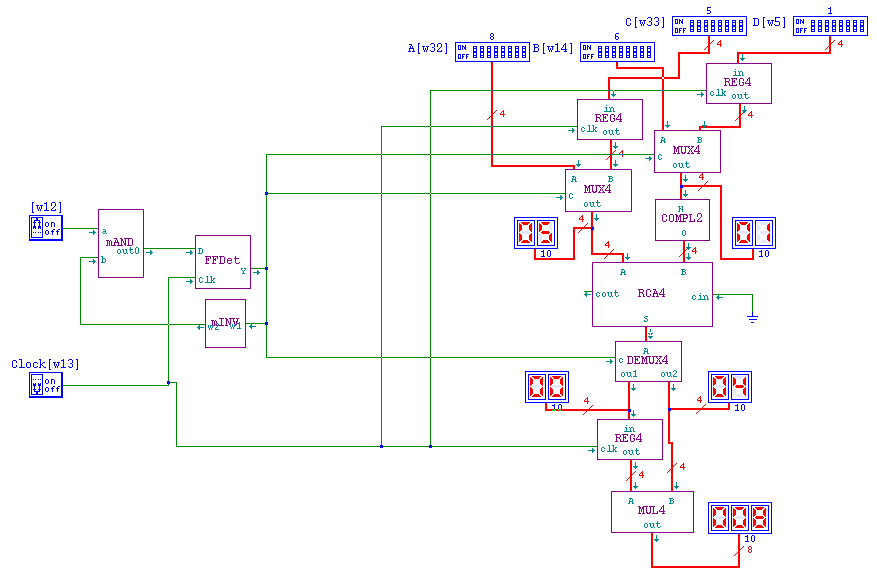
\includegraphics[width=\textwidth]{s2c1}
    \caption{Simulazione 2: ciclo di clock 1}
    \label{ }
    \end{minipage}
\end{figure}

\begin{figure}[H]
    \begin{minipage}[c]{\textwidth}
    \centering
    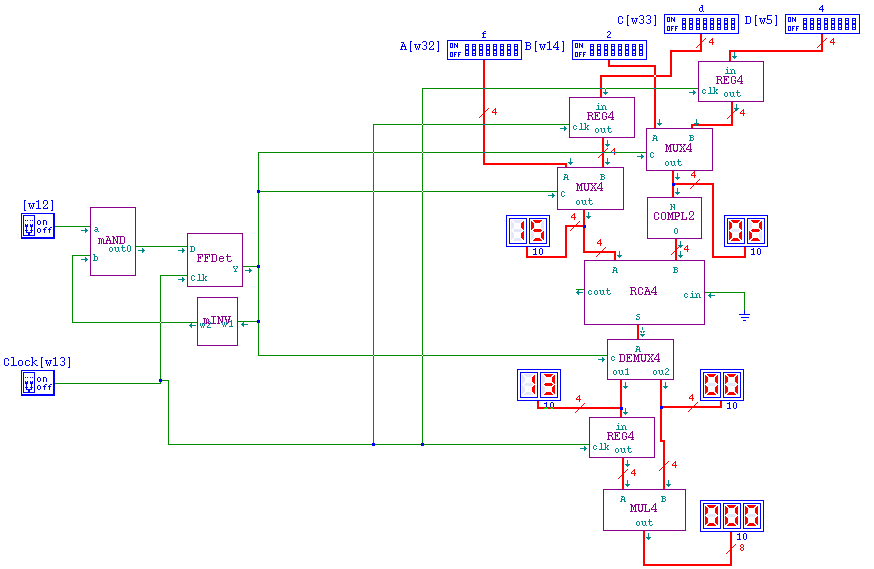
\includegraphics[width=\textwidth]{s3c0}
    \caption{Simulazione 3: ciclo di clock 0}
    \label{ }
    \end{minipage}
\end{figure}

\begin{figure}[H]
    \begin{minipage}[c]{\textwidth}
    \centering
    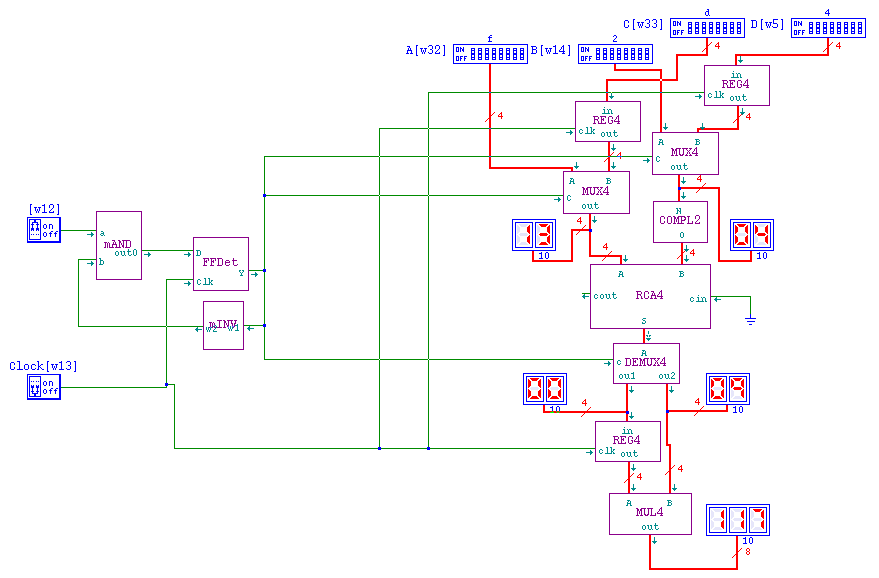
\includegraphics[width=\textwidth]{s3c1}
    \caption{Simulazione 3: ciclo di clock 1}
    \label{ }
    \end{minipage}
\end{figure}

\subsection{Stima di complessità circuitale e prestazioni}
Per valutare le prestazioni del circuito finale, è necessario introdurre quattro metriche: \emph{complessità circuitale (\textbf{Area}), \textbf{tempo di propagazione} (il tempo necessario per stabilizzare le uscite), 
\textbf{tempo di contaminazione} (il tempo necessario affinchè si verifichi la prima variazione delle uscite)}, e \emph{\textbf{latenza} (numero di risultati producibili nell'unità di tempo)}.
E' dunque necessario stimare ciascuna di queste metriche per ognuno dei componenti del circuito partendo dal livello gate, dunque dalle porte logiche (semplici e composte).
Ognuna di queste metriche viene stimata utilizzando un modello unitario, ovvero ogni porta logica semplice (NOT, NAND e NOR) vale 1.
Il tempo di propagazione si calcola stimando il percorso più lungo che i segnali in ingresso devono seguire, il tempo di contaminazione stimando quello più breve, mentre l'area corrisponde semplicemente
al numero di porte logiche semplici utilizzate per realizzare il componente.

\subsubsection{Prestazioni porte logiche}
\begin{table}[H]
    \begin{minipage}[c]{\textwidth}
    \centering
    \begin{tabular}{|c|c|c|c|c|c|c|}
    \hline
                  & \small{\textbf{NOT}} & \textbf{NAND} & \textbf{NOR} & \textbf{AND}       & \textbf{OR}       & \textbf{EXOR}         \\ \hline
    \textbf{Area} & 1                    & 1             & 1            & A(NAND)+A(NOT)=2   & A(NOR)+A(NOT)=2   & 2*A(NOT)+3*A(NAND)=5  \\ 
    \textbf{Tp}   & 1                    & 1             & 1            & Tp(NAND)+Tp(NOT)=2 & Tp(NOR)+Tp(NOT)=2 & Tp(NOT)+2*Tp(NAND)=3  \\ 
    \textbf{Tc}   & 1                    & 1             & 1            & Tc(NAND)+Tc(NOT)=2 & Tc(NOR)+Tc(NOT)=2 & 2*Tc(NAND)=2          \\ \hline
    \end{tabular}
\end{minipage}
\end{table}

\subsubsection{Prestazioni multiplexer/demultiplexer}
L'area di un multiplexer o demultiplexer a $n$ bit è dipendente linearmente dal numero di bit degli ingressi e delle uscite, in quanto serve un MUX per ciascun bit.
Il tempi di propagazione e contaminazione non sono invece dipendenti dal numero di bit degli ingressi, in quanto i bit delle uscite vengono tutti selezionati in parallelo. Dunque i tempi
di propagazione e contaminazione sono gli stessi dei multiplexer/demultiplexer a 1 bit.

\begin{table}[H]
    \begin{minipage}[c]{\textwidth}
    \centering
        \begin{tabular}{|c|c|c|c|c|c|c|}
        \hline
                      & \textbf{MUX}               & \textbf{MUX 4 BIT} & \textbf{DEMUX}     & \textbf{DEMUX 4 BIT} \\ \hline
        \textbf{Area} & 2*A(AND)+A(OR)+A(NOT) = 7  & 4*A(MUX) = 28      & 2*A(AND)+A(INV)=5  & 4*A(DEMUX)=20        \\ 
        \textbf{Tp}   & Tp(NOT)+Tp(AND)+Tp(OR) = 5 & Tp(MUX) = 5        & Tp(NOT)+Tp(AND)=3  & Tp(DEMUX)=3          \\ 
        \textbf{Tc}   & Tc(AND)+Tc(OR) = 4         & Tc(MUX) = 4        & Tc(AND)=2          & Tc(DEMUX)=2          \\ \hline
        \end{tabular}
    \end{minipage}
\end{table}

\subsubsection{Prestazioni registri}
Gli elementi di memoria che memorizzano un solo bit (latch e flip-flop) non hanno dipendendenza dal numero degli operandi.
Per i registri parallelo/parallelo, invece, l'area dipende linearmente dal numero di bit da memorizzare.
I tempi di propagazione e contaminazione non hanno dipendenza dal numero di bit da memorizzare, in quanto scrittura e lettura avvengono in parallelo per ciascun bit, dunque sia Tp che Tc sono pari
a quelli di un singolo FF D edge triggered.

\begin{table}[H]
    \begin{minipage}[c]{\textwidth}
    \centering
        \begin{tabular}{|c|c|c|c|c|c|c|}
        \hline
                      & \textbf{LatchSR}  & \textbf{FFSR}      & \textbf{FFDls}     & \textbf{FFDet}         & \textbf{Registri 4 bit} \\ \hline
        \textbf{Area} & 2*A(NOR) = 2      & A(LSR)+2*A(AND)=6  & A(FFSR)+A(INV)=7   & 2*A(FFDls)+A(NOT)=15   & 4*A(FFDet)=60           \\ 
        \textbf{Tp}   & Tp(NOR) = 2       & Tp(LSR)+Tp(AND)=4  & Tp(NOT)+Tp(FFSR)=5 & 2*Tp(FFDls)+Tp(INV)=11 & Tp(FFDet)=11            \\ 
        \textbf{Tc}   & Tc(NOR) = 1       & Tc(NOR)+Tc(AND)=3  & Tc(FFSR)=3         & Tc(FFDls)=3            & Tc(FFDet)=3             \\ \hline
        \end{tabular}
    \end{minipage}
\end{table}

\subsubsection{Prestazioni macro aritmetiche}
\begin{itemize}
\item \textbf{Half Adder e Full Adder:}
    \begin{itemize}
        \item Il tempo di propagazione dell'HA corrisponde al tempo di propagazione massimo tra quello della porta AND e della porta EXOR, in quanto le due non sono collegate l'una all'altra
        ma calcolano i risultati in maniera indipendente. Analogamente, il tempo di contaminazione è quello minore tra i tempi di contaminazione delle due porte.
        \item Il tempo di propagazione del FA corrisponde al tempo necessario ad attraversare i due HA e la porta OR; mentre il tempo di contaminazione è quello di un singolo HA, in quanto il percorso 
        più breve è quello tra il riporto in ingresso e l'uscita del bit di somma.
    \end{itemize}
    
    \begin{table}[H]
        \begin{minipage}[c]{\textwidth}
        \centering
        \begin{tabular}{|c|c|c|c|c|}
        \hline
                      & \textbf{HA}              & \textbf{FA}       \\ \hline
        \textbf{Area} & A(AND)+A(EXOR)=7         & 2*A(HA)+A(OR)=16  \\ 
        \textbf{Tp}   & max(Tp(AND), Tp(EXOR))=3 & 2*Tp(HA)+Tp(OR)=8 \\ 
        \textbf{Tc}   & min(Tc(AND),Tc(EXOR))=2  & Tc(HA)=2          \\ 
        \textbf{Rate} & 1/Tp(HA)                 & 1/Tp(FA)          \\ \hline
        \end{tabular}
    \end{minipage}
    \end{table}

\item \textbf{Complementatore a 4 bit:}\\
    L'area del complementatore è quadraticamente dipendente dal numero degli operandi, in quanto per ogni bit degli ingressi sono necessari un HA e una porta NOT:\\
    A(C2n) = $n$*A(HA) + $n$*A(NOT) = $O(n^2)$.
    Il percorso più lungo corrisponde al caso in cui il riporto in uscita si propaghi dal primo all'ultimo HA, dunque il tempo di propagazione totale dipende linearmente dal numeri di bit del valore
    da complementare.
    Tp(C2n) = Tp(NOT) + $n$*Tp(HA) = $O(n)$.
    Il percorso più breve è quello che attraversa un singolo invert e un singolo HA.
    
    \begin{table}[H]
        \begin{minipage}[c]{\textwidth}
        \centering
        \begin{tabular}{|c|c|c|c|c|}
        \hline
                      & \textbf{C2}           \\ \hline
        \textbf{Area} & 4*A(HA)+4*A(NOT)=32   \\ 
        \textbf{Tp}   & 4*Tp(HA)+Tp(NOT)=13   \\ 
        \textbf{Tc}   & Tc(HA)+Tc(NOT)=3      \\ 
        \textbf{Rate} & 1/Tp(C2)              \\ \hline
        \end{tabular}
    \end{minipage}
    \end{table}
    
\item \textbf{RCA4:}\\
    L'area del RCA, così come il tempo di propagazione, dipendono linearmente dal numero di bit degli operandi, in quanto è necessario un FA per ogni coppia di bit. 
    Il tempo di contaminazione è invece sempre pari a quello di un FA.

    \begin{table}[H]
        \begin{minipage}[c]{\textwidth}
        \centering
        \begin{tabular}{|c|c|c|c|c|}
        \hline
                      & \textbf{RCA4}  \\ \hline
        \textbf{Area} & 4*A(FA)=64     \\ 
        \textbf{Tp}   & 4*Tp(FA)=32    \\ 
        \textbf{Tc}   & Tc(FA)=2       \\ 
        \textbf{Rate} & 1/Tp(RCA)=0.03 \\ \hline
        \end{tabular}
    \end{minipage}
    \end{table}
    
\textbf{Moltiplicatore:}\\
Il moltiplicatore descritto in precedenza conta in totale 16 porte AND per il calcolo dei prodotti tra singoli bit, 2 HA e 8 FA. L'area corrisponde quindi alla somma delle aree dei componenti elencati.
Il percorso più lungo che i segnali in ingresso devono percorrere è quello dei due bit in ingresso al primo HA, nel caso in cui ci sia sempre in riporto in uscita da propagare alla colonna successiva,
e dunque il segnale attraversa tutti i full-adder e half-adder.
Il percorso più breve è invece quello del prodotto tra i primi due bit di ciascun moltiplicando, che non devono essere sommati ad altri prodotti, e dunque attraversano una sola porta AND.

\begin{table}[H]
    \begin{minipage}[c]{\textwidth}
    \centering
    \begin{tabular}{|c|c|c|}
    \hline
                  & \textbf{MUL4}                   \\ \hline
    \textbf{Area} & 16*A(AND)+8*A(FA)+2*A(HA)=174   \\ 
    \textbf{Tp}   & 2*Tp(AND)+2*Tp(HA)+8*Tp(FA)=74  \\ 
    \textbf{Tc}   & Tc(AND)=2                       \\ 
    \textbf{Rate} & >1/Tp(MUL)=0.01                 \\ \hline
    \end{tabular}
\end{minipage}
\end{table}
\end{itemize}

\subsubsection{Circuito Completo}
\begin{itemize}
\item L'area del circuito completo è costituita dalla somma delle aree di tutti i suoi componenti.
      \textbf{A(TOT)} = 2*A(MUX)+A(C2)+A(DEMUX)+A(RCA4)+A(MUL4)+3*A(REG4) = 526\\

\item Il percorso più lungo all'interno del circuito è quello dei sottraendi, che attraversano tutti i componenti del circuito. 
      Il tempo di propagazione corrisponde dunque alla sommma dei Tp dei suoi componenti.\\
      \textbf{Tp(TOT)} = Tp(MUX)+Tp(RCA4)+Tp(DEMUX)+Tp(MUL4)+Tp(C2)+Tp(REG4) = 149\\

\item Il percorso più breve è quello dei minuendi, che non attraversano il complementatore.\\
      \textbf{Tc(TOT)} = 2*Tc(MUX)+Tc(DEMUX)+Tc(RCA4)+Tc(MUL4)+3*Tc(REG4) = 32\\
\end{itemize}

Quindi la durata minima che il ciclo di clock può assumere è pari a quella necessaria a completare il secondo ciclo di clock, in quanto durante il primo non viene eseguita la moltiplicazione.
Il tempo necessario a concludere i calcoli per il secondo ciclo di clock è uguale al tempo di propagazione totale del circuito, più il tempo di propagazione del registro contenente il risultato
del primo ciclo di clock.\\ 

\textbf{TClock > Tp(TOT) + Tp(REG4) = 160}\\

I tempi di propagazione e contaminazione sono stati stimati sul circuito completo tramite simulazione:

\begin{figure}[ht]
    \begin{minipage}[c]{\textwidth}
    \centering
    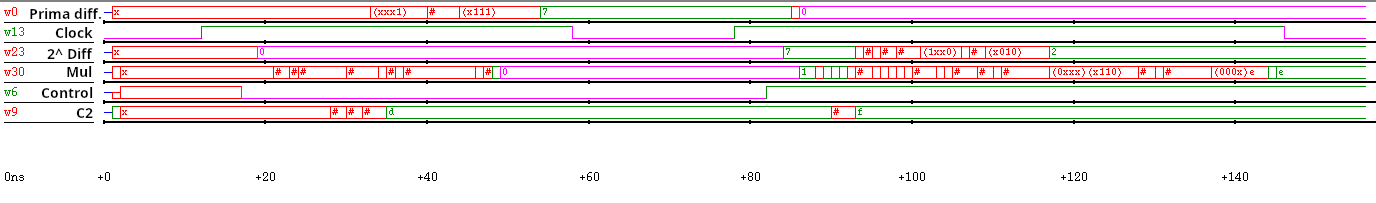
\includegraphics[width=\textwidth]{onda}
    \caption{Simulazione dei tempi di propagazione e contaminazione}
    \label{ }
    \end{minipage}
\end{figure}

Osservando l'immagine sopra riportata, e assumendo di far corrispondere il modello unitario precedentemente adottato ad 1ns, è possibile stabilire che i tempi di propagazione e contaminazione corrispondono,
con ragionevole approssimazione, a quelli stimati.


\end{document}